% Options for packages loaded elsewhere
\PassOptionsToPackage{unicode}{hyperref}
\PassOptionsToPackage{hyphens}{url}
\documentclass[
  ignorenonframetext,
]{beamer}
\newif\ifbibliography
\usepackage{pgfpages}
\setbeamertemplate{caption}[numbered]
\setbeamertemplate{caption label separator}{: }
\setbeamercolor{caption name}{fg=normal text.fg}
\beamertemplatenavigationsymbolsempty
% remove section numbering
\setbeamertemplate{part page}{
  \centering
  \begin{beamercolorbox}[sep=16pt,center]{part title}
    \usebeamerfont{part title}\insertpart\par
  \end{beamercolorbox}
}
\setbeamertemplate{section page}{
  \centering
  \begin{beamercolorbox}[sep=12pt,center]{section title}
    \usebeamerfont{section title}\insertsection\par
  \end{beamercolorbox}
}
\setbeamertemplate{subsection page}{
  \centering
  \begin{beamercolorbox}[sep=8pt,center]{subsection title}
    \usebeamerfont{subsection title}\insertsubsection\par
  \end{beamercolorbox}
}
% Prevent slide breaks in the middle of a paragraph
\widowpenalties 1 10000
\raggedbottom
\AtBeginPart{
  \frame{\partpage}
}
\AtBeginSection{
  \ifbibliography
  \else
    \frame{\sectionpage}
  \fi
}
\AtBeginSubsection{
  \frame{\subsectionpage}
}
\usepackage{iftex}
\ifPDFTeX
  \usepackage[T1]{fontenc}
  \usepackage[utf8]{inputenc}
  \usepackage{textcomp} % provide euro and other symbols
\else % if luatex or xetex
  \usepackage{unicode-math} % this also loads fontspec
  \defaultfontfeatures{Scale=MatchLowercase}
  \defaultfontfeatures[\rmfamily]{Ligatures=TeX,Scale=1}
\fi
\usepackage{lmodern}
\ifPDFTeX\else
  % xetex/luatex font selection
\fi
% Use upquote if available, for straight quotes in verbatim environments
\IfFileExists{upquote.sty}{\usepackage{upquote}}{}
\IfFileExists{microtype.sty}{% use microtype if available
  \usepackage[]{microtype}
  \UseMicrotypeSet[protrusion]{basicmath} % disable protrusion for tt fonts
}{}
\makeatletter
\@ifundefined{KOMAClassName}{% if non-KOMA class
  \IfFileExists{parskip.sty}{%
    \usepackage{parskip}
  }{% else
    \setlength{\parindent}{0pt}
    \setlength{\parskip}{6pt plus 2pt minus 1pt}}
}{% if KOMA class
  \KOMAoptions{parskip=half}}
\makeatother
\usepackage{graphicx}
\makeatletter
\newsavebox\pandoc@box
\newcommand*\pandocbounded[1]{% scales image to fit in text height/width
  \sbox\pandoc@box{#1}%
  \Gscale@div\@tempa{\textheight}{\dimexpr\ht\pandoc@box+\dp\pandoc@box\relax}%
  \Gscale@div\@tempb{\linewidth}{\wd\pandoc@box}%
  \ifdim\@tempb\p@<\@tempa\p@\let\@tempa\@tempb\fi% select the smaller of both
  \ifdim\@tempa\p@<\p@\scalebox{\@tempa}{\usebox\pandoc@box}%
  \else\usebox{\pandoc@box}%
  \fi%
}
% Set default figure placement to htbp
\def\fps@figure{htbp}
\makeatother
\setlength{\emergencystretch}{3em} % prevent overfull lines
\providecommand{\tightlist}{%
  \setlength{\itemsep}{0pt}\setlength{\parskip}{0pt}}
% Slide layout defaults for warning-clean scientific decks.
\usepackage{etoolbox}
\IfFileExists{xurl.sty}{\usepackage{xurl}}{}
\IfFileExists{seqsplit.sty}{\usepackage{seqsplit}}{\newcommand{\seqsplit}[1]{#1}}
\protected\def\breakseq#1{\seqsplit{#1}}
\protected\def\breaktt#1{\begingroup\ttfamily\seqsplit{#1}\endgroup}
\setlength{\emergencystretch}{6em}
\tolerance=5000
\hbadness=10000
\hfuzz=1pt
\setlength{\tabcolsep}{2pt}
\AtBeginEnvironment{longtable}{\tiny\renewcommand{\arraystretch}{0.86}\setlength{\tabcolsep}{1pt}}
\AtBeginEnvironment{tabular}{\tiny\renewcommand{\arraystretch}{0.86}\setlength{\tabcolsep}{1pt}}

% Natbib and cross-reference fallbacks — slides don't load natbib
% or cleveref, but combined-PDF manuscript prose may emit these
% commands. The fallback renders citations as a bracketed key list
% and cross-references as detokenized labels so slides don't fail on
% undefined control sequences or raw underscores. \providecommand is
% a no-op if packages load later.
\providecommand{\citep}[1]{[#1]}
\providecommand{\citet}[1]{#1}
\providecommand{\citealp}[1]{#1}
\providecommand{\citeauthor}[1]{#1}
\providecommand{\citeyear}[1]{#1}
\providecommand{\cref}[1]{\texttt{\detokenize{#1}}}
\providecommand{\Cref}[1]{\texttt{\detokenize{#1}}}

\newtheorem{proposition}{Proposition}
\newtheorem{hypothesis}{Hypothesis}
\usepackage{bookmark}
\IfFileExists{xurl.sty}{\usepackage{xurl}}{} % add URL line breaks if available
\urlstyle{same}
% fallback for those not using the hyperref driver hyperxmp:
\makeatletter
\@ifundefined{xmpquote}{\newcommand{\xmpquote}[1]{#1}}{}
\makeatother
\hypersetup{
  hidelinks,
  pdfcreator={LaTeX via pandoc}}

\author{\texorpdfstring{}{}}
\date{}

\begin{document}

\section{Neuroergonomic Burden and Shared
Attention}\label{sec:neuroergonomics}

\begin{frame}[fragile,allowframebreaks]{Neuroergonomic Burden and Shared
Attention}
Neuroergonomics studies brain and behavior in real-world tasks rather
than only laboratory tasks \breakseq{[@ayaz2019neuroergonomics]}. DigiPPPiP
needs this framing because the desired practice happens in homes, cafes,
studios, hospitals, classrooms, and long-distance relationships. Mobile
functional near-infrared spectroscopy (fNIRS) and related field methods
make it increasingly plausible to study social and cognitive workload in
naturalistic environments \breakseq{[@dehais2020grand;
@moffat2024mobilefnirs]}. The same literature also cautions that
naturalism raises measurement risk: motion, lighting, posture, fatigue,
device familiarity, and partner relationship history can all change what
a signal means.

The core design rule is restraint. The original paper-based practice
worked partly because the interface was nearly invisible: pen, paper,
partner, mark \breakseq{[@mikhailova2018pppip]}. Digital implementations should
add capabilities only where they support the dyad: shared visibility,
accessibility, persistence, consentful replay, or place anchoring. Tool
palettes, notifications, social feeds, and AI suggestions can easily
become technoference if they compete with partner attention, a risk
already documented in couple-relationship technology research
\breakseq{[@mcdaniel2016technoference]}.

Attention is the scarce resource in DigiPPPiP. The first-principles
question for any interface feature is whether it increases
partner-directed perception, action, repair, or reflection. A feature
that increases expressivity while fragmenting attention is not
automatically an improvement. A slower or plainer interface may be
neuroergonomically superior when it keeps the dyad inside the shared act
rather than inside the tool.

\breakseq{[@fig:neuroergonomics\_flow]} operationalizes three design
constraints. The flow surface represents challenge-skill balance,
drawing on flow research while remaining a conceptual interface
diagnostic rather than an experience sample
\breakseq{[@csikszentmihalyi1989flow]}. The technoference curve models the cost
of interruptions. The attention simplex asserts that attention must be
allocated among the partner's marks, one's own marks, and the shared
canvas. These are design diagnostics, not biomarkers. Their purpose is
to make interface burden visible before a digital feature is treated as
relationally helpful.

\begin{figure}
\centering
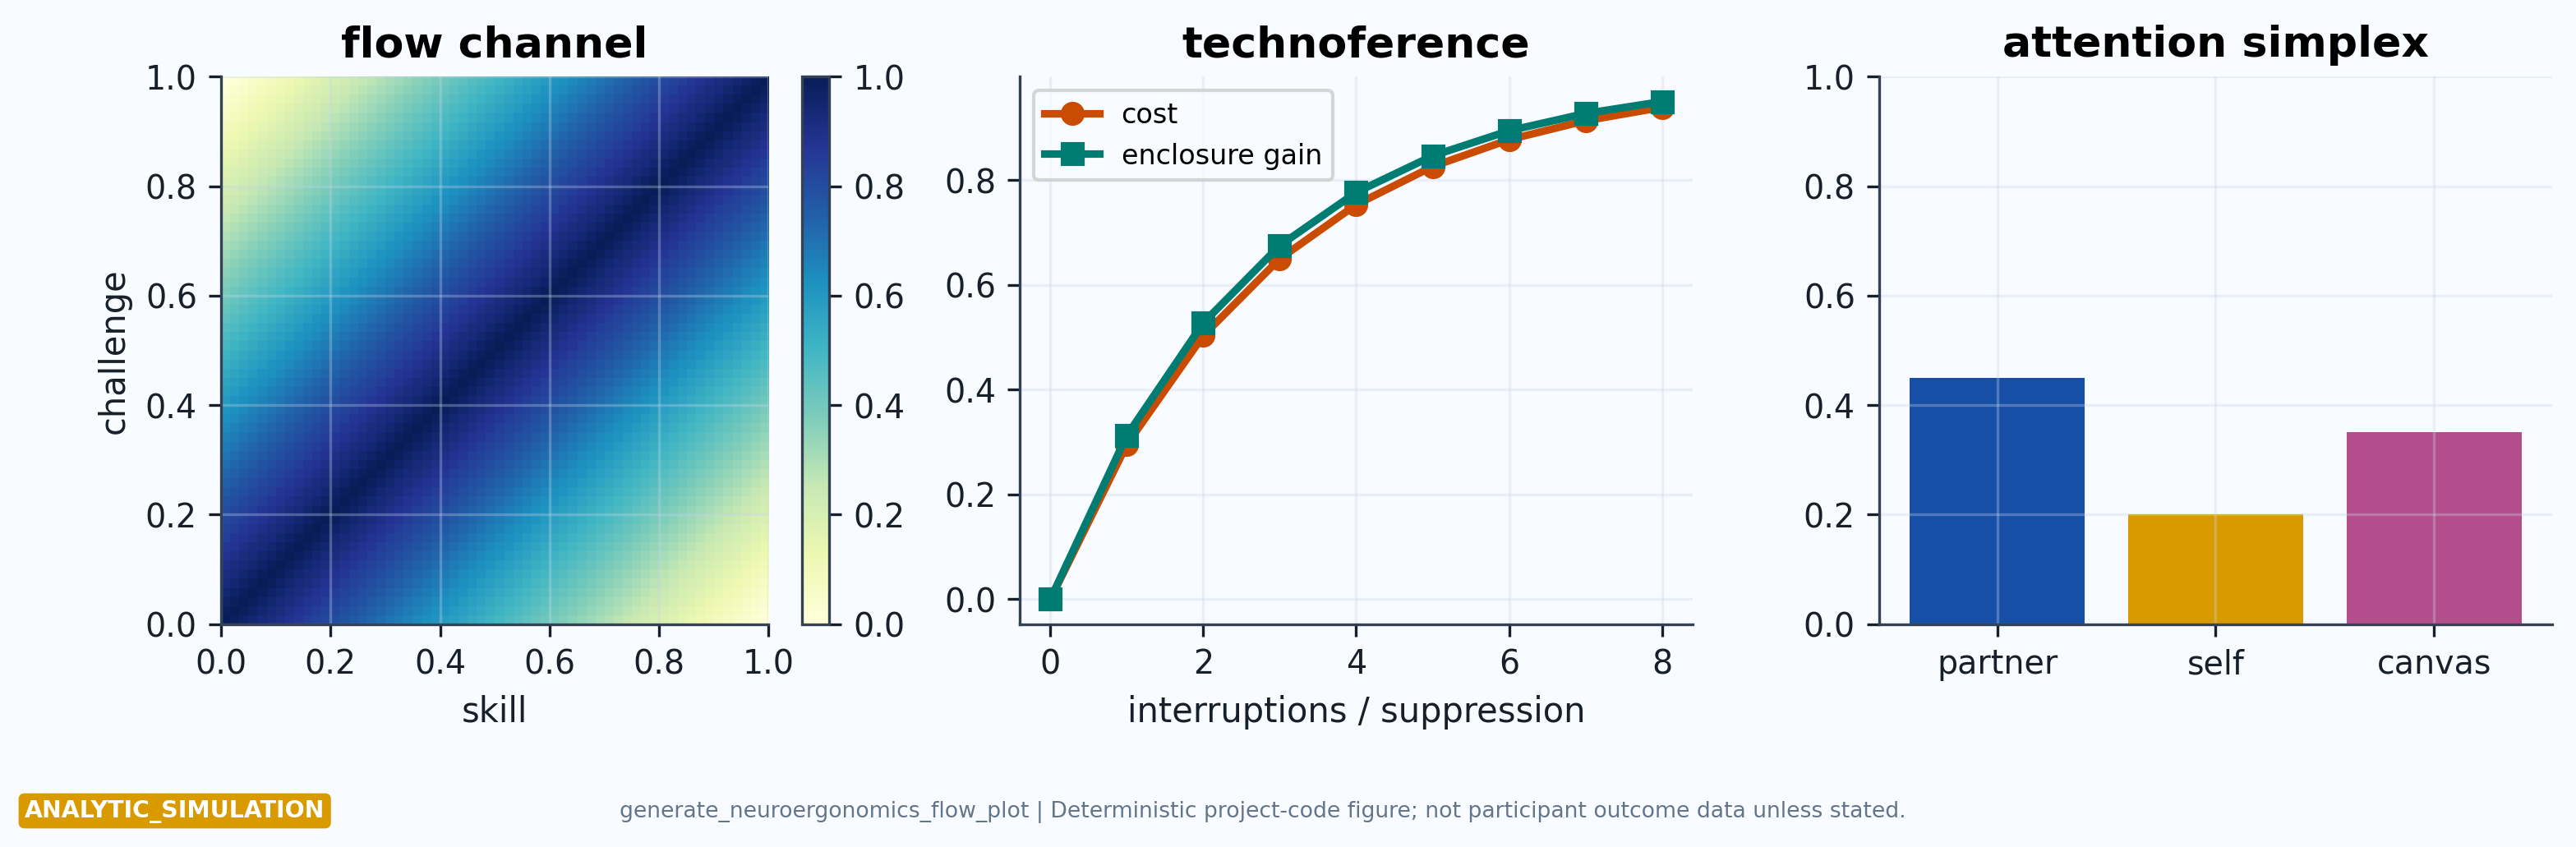
\includegraphics[width=0.9\linewidth,height=0.46\textheight,keepaspectratio,alt={Conceptual neuroergonomic diagnostics: flow channel, technoference cost, intentional-enclosure gain, and attention allocation. The figure is generated by generate\_neuroergonomics\_flow\_plot() from src/neuroergonomics.py; read the panels as challenge-skill fit, interruption cost versus enclosure gain, and distribution of attention across partner, self, and canvas. It supports interface-burden reasoning. The values are design primitives, not measured workload or flow-state evidence.}]{../figures/neuroergonomics_flow.png}
\caption{Conceptual neuroergonomic diagnostics: flow channel,
technoference cost, intentional-enclosure gain, and attention
allocation. The figure is generated by
\protect\breaktt{generate\_neuroergonomics\_flow\_plot()} from
\protect\breaktt{src/neuroergonomics.py}; read the panels as
challenge-skill fit, interruption cost versus enclosure gain, and
distribution of attention across partner, self, and canvas. It supports
interface-burden reasoning. The values are design primitives, not
measured workload or flow-state
evidence.}\label{fig:neuroergonomics_flow}
\end{figure}

Brain-computer interface (BCI) and neurofeedback extensions should
remain secondary to the human-human practice. Digital art-therapy
research suggests that technology can support creative expression and
research instrumentation while creating ethical, material, and access
constraints \breakseq{[@zubala2021digitalarttherapy; @reitere2024telehealth]},
but DigiPPPiP should not make neural instrumentation a prerequisite. The
strongest design path is progressive enhancement: the practice works
with pen and paper, improves with a shared digital canvas, and may later
support optional biofeedback for research contexts.
\end{frame}

\end{document}
